% Created 2014-10-27 星期一 17:09
\documentclass{article}
\usepackage{fixltx2e}
\usepackage{graphicx}
\usepackage{longtable}
\usepackage{float}
\usepackage{wrapfig}
\usepackage{soul}
\usepackage{textcomp}
\usepackage{marvosym}
\usepackage{wasysym}
\usepackage{latexsym}
\usepackage{amssymb}
\usepackage{hyperref}
\tolerance=1000
\usepackage{etex}
\usepackage{amsmath}
\usepackage{pstricks}
\usepackage{pgfplots}
\usepackage{tikz}
\usepackage[europeanresistors,americaninductors]{circuitikz}
\usepackage{colortbl}
\usepackage{yfonts}
\usetikzlibrary{shapes,arrows}
\usetikzlibrary{positioning}
\usetikzlibrary{arrows,shapes}
\usetikzlibrary{intersections}
\usetikzlibrary{calc,patterns,decorations.pathmorphing,decorations.markings}
\usepackage[BoldFont,SlantFont,CJKchecksingle]{xeCJK}
\setCJKmainfont[BoldFont=Evermore Hei]{Evermore Kai}
\setCJKmonofont{Evermore Kai}
\usepackage{pst-node}
\usepackage{pst-plot}
\psset{unit=5mm}
\usepackage{beamerarticle}
\mode<beamer>{\usetheme{Frankfurt}}
\mode<beamer>{\usecolortheme{dove}}
\mode<article>{\hypersetup{colorlinks=true,pdfborder={0 0 0}}}
\mode<beamer>{\AtBeginSection[]{\begin{frame}<beamer>\frametitle{Topic}\tableofcontents[currentsection]\end{frame}}}
\setbeamercovered{transparent}
\providecommand{\alert}[1]{\textbf{#1}}

\title{线性系统的根轨迹法}
\author{}
\date{}
\hypersetup{
  pdfkeywords={},
  pdfsubject={},
  pdfcreator={Emacs Org-mode version 7.9.3f}}

\begin{document}

\maketitle

\begin{frame}
\frametitle{Outline}
\setcounter{tocdepth}{3}
\tableofcontents
\end{frame}













\section{基本概念}
\label{sec-1}
\subsection{零极点与根轨迹}
\label{sec-1-1}
\begin{frame}
\frametitle{根轨迹法}
\label{sec-1-1-1}

\begin{itemize}
\item <2->系统性能由闭环极点决定
\item <3->目的:分析系统参数变化对系统性能影响
\item <4->根轨迹法:根据系统开环零极点作出系统闭环极点随参数变动的轨迹
\end{itemize}
\end{frame}
\begin{frame}
\frametitle{分析 $K$ 变化对系统性能的影响}
\label{sec-1-1-2}


\begin{tikzpicture}[node distance=2em,auto,>=latex', thick]
%\path[use as bounding box] (-1,0) rectangle (10,-2); 
\path[->] node[] (r) { $ r(t) $ }; 
\path[->] node[ circle,inner sep=2pt,minimum size=1pt,draw,label=below left: $   $ ,right =of r] (p1) { }; 
\path[->](r) edge node {} (p1) ; 
%\path[red] node[draw, right =of p1] (n) { $ N $ }; 
%\path[->] (p1) edge node[midway] { $ x(t) $ } (n) ; 
\path[red] node[draw, inner sep=5pt,right =of p1] (g) { $ \frac{K}{s(s+1)} $ }; 
\path[->] (p1) edge node [midway]{ $   $ } (g); 
\path[->] node[ right =of g] (o) { $ c(t) $ }; 
\path[->] (g) edge node {} (o); 
\path[->, draw] (g.east)+(1em,0) -- +(1em,-3em) -| node[very near end] { $ - $ } (p1); 
\end{tikzpicture} 

\begin{eqnarray*}
\Phi(s) & = &\frac{K}{s^2+s+K} \\
D(s) &=& s^2+s+K \\
D(s) &=& 0 \\
s_{1,2} &=& \frac{-1\pm\sqrt{1-4K}}{2}
\end{eqnarray*}

\mode<beamer>{\rowcolors[]{1}{green!10}{blue!10}}
\begin{tabular}{l!{\vrule}c<{\onslide<2->}c<{\onslide<3->}c<{\onslide<4->}c<{\onslide<5->}c<{\onslide<6->}c<{\onslide<7->}}
K   & 0  &  0.25 & 1          & 4         & $\cdots$ & $\infty$ \\
$s_1$ & 0  &  -0.5 & -0.5+0.87j & -0.5+1.9j & $\cdots$ & -0.5+ $\infty$ j \\
$s_1$ & -1 &  -0.5 & -0.5-0.87j & -0.5-1.9j & $\cdots$ & -0.5- $\infty$ j 
\end{tabular}
\end{frame}
\subsection{根轨迹的基本条件}
\label{sec-1-2}
\begin{frame}
\frametitle{根轨迹条件:系统模型}
\label{sec-1-2-1}


\begin{tikzpicture}[node distance=2em,auto,>=latex', thick]
%\path[use as bounding box] (-1,0) rectangle (10,-2); 
\path[->] node[] (r) { $ r(t) $ }; 
\path[->] node[ circle,inner sep=2pt,minimum size=1pt,draw,label=below left: $   $ ,right =of r] (p1) { }; 
\path[->](r) edge node {} (p1) ; 
%\path[red] node[draw, right =of p1] (n) { $ N $ }; 
%\path[->] (p1) edge node[midway] { $ x(t) $ } (n) ; 
\path[red] node[draw, inner sep=5pt,right =of p1] (g) { $ G(s) $ }; 
\path[->] (p1) edge node [midway]{ $   $ } (g); 
\path[->] node[ right =of g] (o) { $ c(t) $ }; 
\path[->] (g) edge node {} (o); 
\path[red] node[draw, inner sep=5pt,below =of g] (h) { $ H(s) $ }; 
\path[->,draw] (g.east)+(1em,0) |- (h.east); 
\path[->, draw] (h) -| node[very near end] { $ - $ } (p1); 
%\path[->, draw] (g.east)+(1em,0) -- +(1em,-3em) -| node[very near end] { $ - $ } (p1); 
\end{tikzpicture} 

\begin{itemize}
\item <2-> 开环传递函数(零极点形式):  
          \[G(s)=\frac{K_g\prod_{i=1}^m(s-z_i)}{\prod_{j=1}^n(s-p_j)}\]
\item <3-> 变动的参数:根轨迹增益  $K_g$
\item <4-> $K_g$ 从  $0\rightarrow\infty$  时,闭环极点的运动轨迹
\item <5-> 对于负反馈系统,称为  $180^\circ$  根轨迹.
\end{itemize}
\end{frame}
\begin{frame}
\frametitle{根轨迹条件:幅值条件与相角条件}
\label{sec-1-2-2}


\begin{eqnarray*}
\Phi(s) &=& \frac{G(s)}{1+G(s)H(s)} \\
D(s) &= &1+G(s)H(s) 
     = 0 \\
G(s)H(s) &=& -1 \\
\frac{K_g\prod_{i=1}^m(s-z_i)}{\prod_{j=1}^n(s-p_j)} &=& -1 
\end{eqnarray*}

\begin{itemize}
\item <2->幅值条件:  $\frac{K_g\prod_{i=1}^m|s-z_i|}{\prod_{j=1}^n|s-p_j|} = 1$
\item <3->相角条件:  $\sum_{i=1}^m\angle (s-z_i)-\sum_{j=1}^n\angle (s-p_j) = (2k+1)\pi$
\item <4->命题
\begin{itemize}
\item <4->满足相角条件的点一定是根轨迹上的点
\item <5->根轨迹上的点何时成为系统闭环极点由  $K_g$  决定
\end{itemize}
\item <6->结论: 绘制根轨迹只依据相角条件即可
\end{itemize}
\end{frame}
\section{绘制根轨迹图的基本原则}
\label{sec-2}
\subsection{根轨迹图绘制法则}
\label{sec-2-1}
\begin{frame}
\frametitle{根轨迹图的绘制}
\label{sec-2-1-1}

\begin{itemize}
\item 前提条件:
\begin{itemize}
\item <2->变动参数为开环传递函数的根轨迹增益  $K_g,(K^*)$
\item <3->系统为负反馈系统
\end{itemize}
\item 目的:
\begin{itemize}
\item 根据开环零极点分布绘制闭环极点的运动轨迹
\end{itemize}
\end{itemize}
\end{frame}
\begin{frame}
\frametitle{根轨迹的起点,终点及分支数}
\label{sec-2-1-2}

\begin{itemize}
\item <2->根轨迹起源于开环极点,
\item <3->根轨迹终止于开环零点,
\item <4->有  $\max(m,n)$  条分支,
\item <5->有 $n-m$ 条分支趋向无穷远处.
\end{itemize}
\end{frame}
\begin{frame}
\frametitle{根轨迹的对称性}
\label{sec-2-1-3}

\begin{itemize}
\item <2->根轨迹对称于实轴
\end{itemize}
\end{frame}
\begin{frame}
\frametitle{实轴上的根轨迹}
\label{sec-2-1-4}

\begin{itemize}
\item <2->实轴上某区域若其右边开环实数零极点个数之和为奇数,则该区域为根轨迹区域
\item <2->例:  
     \[G_o(s)=\frac{K_g(s+1)(s+3)}{s(s+2)}\]
\begin{itemize}
\item <3-> 实轴上根轨迹区域:  
             \[ [0,-1],[-2,-3] \]
\end{itemize}
\end{itemize}
\end{frame}
\begin{frame}
\frametitle{渐近线}
\label{sec-2-1-5}

\begin{itemize}
\item <2-> $n>m$ 时,渐近线与实轴交点为  $\sigma_a$  ,夹角为  $\phi$  则:
       	\begin{eqnarray*}
       	\sigma_a & = &\frac{\sum_{i=1}^n p_i -\sum_{j=1}^m z_j}{n-m} \\
       	\phi &=& \frac{(2k+1)\pi}{n-m}
       	\end{eqnarray*}
\end{itemize}
\end{frame}
\begin{frame}
\frametitle{分离点与分离角}
\label{sec-2-1-6}

\begin{itemize}
\item <2->分离点: 两条或两条以上根轨迹分支在  $s$  平面上相交又立刻分开的点称为根轨迹的分离点(会合点)
\item <3->分离角: 相邻两条根轨迹分支的夹角
\end{itemize}
\begin{itemize}

\item 分离点计算:
\label{sec-2-1-6-1}%
\begin{eqnarray*}
G(s) & = & \frac{K_g M(s)}{N(s)}\\
D(s) &=& N(s)+K_g M(s) \\
D(s) &=& 0 \\
N(s) &=& - K_g M(s) \\
D'(s) &=& 0 \\
N'(s) &=& -K_g M'(s) \\
M'(s)N(s) &=&M(s)N'(s) \\
\sum_{i=1}^n\frac{1}{d-p_i} &=& \sum_{j=1}^m\frac{1}{d-z_j}
\end{eqnarray*}


\item 分离角计算:\\
\label{sec-2-1-6-2}%
$\theta_d = \frac{(2k+1)\pi}{l}, k=0,1,\cdots,l-1$ , 其中  $l$  为分离点处根轨迹的分支数

\end{itemize} % ends low level
\end{frame}
\begin{frame}
\frametitle{根轨迹的起始角与终止角}
\label{sec-2-1-7}

\begin{itemize}
\item 起始角( $\theta_{p_i}$ ): 根轨迹从开环极点出发时,其切线与正实轴的夹角(出射角)
\item 终止角( $\phi_{z_j}$ ): 根轨迹终止于开环零点时,其切线与正实轴的夹角(入射角)
\end{itemize}
\end{frame}
\begin{frame}
\frametitle{起始角}
\label{sec-2-1-8}

\begin{eqnarray*}
\sum_{l=1}^{m}\angle(s-z_{l})-\sum_{i=1}^{n}\angle(s-p_{i}) & = & (2k+1)\pi\\
s & = & p_{q}+\delta re^{j\theta}\\
\sum_{l=1}^{m}\angle(p_{q}+\delta re^{j\theta}-z_{l})-\sum_{i=1}^{n}\angle(p_{q}+\delta re^{j\theta}-p_{i}) & = & (2k+1)\pi\\
\lim_{\delta r\rightarrow0}\sum_{l=1}^{m}\angle(p_{q}+\delta re^{j\theta}-z_{l})-\sum_{i=1}^{n}\angle(p_{q}+\delta re^{j\theta}-p_{i}) & = & (2k+1)\pi\\
\sum_{l=1}^{m}\angle(p_{q}-z_{l})-\sum_{p_{q}=p_{i}}\theta-\sum_{p_{q}\not=p_{i}}\angle(z_{q}-p_{i}) & = & (2k+1)\pi
\end{eqnarray*}
\end{frame}
\begin{frame}
\frametitle{终止角}
\label{sec-2-1-9}

\begin{eqnarray*}
\sum_{l=1}^{m}\angle(s-z_{l})-\sum_{i=1}^{n}\angle(s-p_{i}) & = & (2k+1)\pi\\
s & = & z_{q}+\delta re^{j\theta}\\
\sum_{l=1}^{m}\angle(z_{q}+\delta re^{j\theta}-z_{l})-\sum_{i=1}^{n}\angle(z_{q}+\delta re^{j\theta}-p_{i}) & = & (2k+1)\pi\\
\lim_{\delta r\rightarrow0}\sum_{l=1}^{m}\angle(z_{q}+\delta re^{j\theta}-z_{l})-\sum_{i=1}^{n}\angle(z_{q}+\delta re^{j\theta}-p_{i}) & = & (2k+1)\pi\\
\sum_{z_{q}\not=z_{l}}\angle(z_{q}-z_{l})+\sum_{z_{q}=z_{l}}\theta-\sum_{i=1}^{n}\angle(z_{q}-p_{i}) & = & (2k+1)\pi
\end{eqnarray*}
\end{frame}
\begin{frame}
\frametitle{根轨迹的起始角与终止角计算公式:}
\label{sec-2-1-10}

   
\begin{eqnarray*}
\theta_{p_i} & = & \frac{(2k+1)\pi}{I}+\frac{1}{I}\left[\sum_{j=1}^m\angle(p_i-z_j)-\sum_{\substack{j=1 \\ p_j\neq p_i}}^n\angle(p_i-p_j)\right] \\
\phi_{z_j} & = & \frac{(2k+1)\pi}{J}-\frac{1}{J}\left[\sum_{\substack{i=1 \\ z_i\neq z_j}}^m\angle(z_j-z_i)-\sum_{i=1}^n\angle(z_j-p_i)\right] 
\end{eqnarray*}
\begin{itemize}
\item $I$ 极点重根个数
\item $J$ 零点重根个数
\end{itemize}
\end{frame}
\begin{frame}
\frametitle{根轨迹的起始角与终止角计算公式(无重根时):}
\label{sec-2-1-11}

   
\begin{eqnarray*}
\theta_{p_i} & = & 180^{\circ}+\left[\sum_{j=1}^m\angle(p_i-z_j)-\sum_{\substack{j=1 \\ j\neq i}}^n\angle(p_i-p_j)\right] \\
\phi_{z_j} & = & 180^{\circ}-\left[\sum_{\substack{i=1 \\ i\neq j}}^m\angle(z_j-z_i)-\sum_{i=1}^n\angle(z_j-p_i)\right] 
\end{eqnarray*}

即:
\begin{itemize}
\item $\theta_{p_i}$  等于:  $180^{\circ}$  +(所有零点指向极点 $p_i$ 的角度之和 -所有其它极点指向极点 $p_i$ 的角度之和)
\item $\phi_{z_i}$ 等于: $180^{\circ}$ -(所有其它零点指向零点 $z_j$ 的角度之和 -所有极点指向零点 $z_j$ 的角度之和)
\end{itemize}
\end{frame}
\begin{frame}
\frametitle{根轨迹与虚轴交点}
\label{sec-2-1-12}
\begin{itemize}

\item 直接计算\\
\label{sec-2-1-12-1}%
将 $s=j\omega$ 代入$D(s)$ ,求出 $K_g,\omega$ , $(0,j\omega)$ 即为交点

\begin{eqnarray*}
D(s) &= &K_gM(s)+N(s) \\
 &=& 0 \\
s &=& j\omega \\
D(j\omega) &=& 0 \\
\Re[D(j\omega)] &=& 0\\
\Im[D(j\omega)] &=& 0
\end{eqnarray*}


\item 利用Routh判据计算\\
\label{sec-2-1-12-2}%
例:
\begin{gather*}
G_o(s)  =  \frac{K_g}{s(s+1)(s+2)} \\
D(s)  = s^3+3s^2+2s+K_g \\
\begin{matrix}
s^3  &  1 &  2 \\
s^2  &  3  &  K_g \\
s^1  & \frac{6-K_g}{3} \\
s^0  & K_g
\end{matrix}
\end{gather*}

令 $\frac{6-K_g}{3}=0$ 得 $K_g=6$, 解辅助方程: $3s^2+K_g=0$ 得 $s=\pm j\sqrt{2}$
\end{itemize} % ends low level
\end{frame}
\begin{frame}
\frametitle{根之和}
\label{sec-2-1-13}

\begin{itemize}
\item <2-> $n-m\geq 2$ 时, 闭环极点之和等于开环极点之和
\end{itemize}
\end{frame}
\subsection{示例}
\label{sec-2-2}
\begin{frame}
\frametitle{根轨迹示例1 $G_o(s) = \frac{K_g(s+1)}{s(s+4)(s^2+2s+2)}$}
\label{sec-2-2-1}


解:
\begin{itemize}
\item <2->开环零点: $-1$ , 开环极点: $0,-4,-1\pm j$
\item <3->实轴上根轨迹:  $[-1,0],[-\infty,-4]$
\item <4->渐近线:
\begin{itemize}
\item $\sigma_a=\frac{\sum p_i-\sum z_j}{n-m}=\frac{-6+1}{3}=-\frac{5}{3}$
\item $\phi=\pm\frac{\pi}{3}$
\end{itemize}
\item <5->起始角:
\begin{itemize}
\item $\theta_{p_1}=180^{\circ}+(90^{\circ}-135^{\circ}-90^{\circ}-\arctan\frac{1}{3})=27^{\circ}$
\item $\theta_{p_2}=-27^{\circ}$
\end{itemize}
\end{itemize}
\end{frame}
\begin{frame}
\frametitle{根轨迹示例1(续)}
\label{sec-2-2-2}

  与虚轴交点  $D(s)=s^4+6s^3+10s^2+(8+K_g)s+K_g =0$ 
\begin{itemize}

\item Routh表如下\\
\label{sec-2-2-2-1}%
\[\begin{matrix}
       	s^4 & 1 & 10 & K_g \\
       	s^3 & 6 & 8+K_g \\
       	s^2 & \frac{52-K_g}{6} & K_g \\
       	s^1 & 8+K_g-\frac{36K_g}{52-K_g} \\
       	s^0 & K_g
       	\end{matrix}\]

\end{itemize} % ends low level
\end{frame}
\begin{frame}
\frametitle{根轨迹示例1(续)}
\label{sec-2-2-3}
\begin{itemize}

\item 计算交点处 $K_g$\\
\label{sec-2-2-3-1}%
\begin{eqnarray*}
       	8+K_g-\frac{36K_g}{52-K_g} &=& 0\\
       	K_g^2-8K_g-416 &=& 0 \\
       	K_g &=& 4\pm 4\sqrt{27} \\
       	\end{eqnarray*}


\item 取 $K_g=4+4\sqrt{27}$ 代入辅助方程:\\
\label{sec-2-2-3-2}%
\begin{eqnarray*}
       	\frac{52-K_g}{6}s^2+K_g & = &0 \\
       	s_{1,2} &=& \pm j2.3
       	\end{eqnarray*}

\end{itemize} % ends low level
\end{frame}
\begin{frame}
\frametitle{根轨迹示例1(续)根轨迹图}
\label{sec-2-2-4}

\begin{tikzpicture}
\coordinate (o) at (0,0);
\coordinate (ox) at (0.5,0);
\draw[->] (-5,0) -- (ox);
\draw[->] (0,-3) -- (0,3);
\draw (o) node[below left] {$o$};
\draw[thick,red] (-4,0) node {$\times$};
\draw[thick,red] (0,0) node {$\times$};
\draw[thick,red] (-1,1) node {$\times$};
\draw[thick,red] (-1,-1) node {$\times$};
\draw[thick,blue] (-1,0) node {$o$};
\draw [red,thick,smooth] plot coordinates {(-1,-1) (-0.5,-1.3) (0,-2.3) (0.5,-3.5)};
\draw [red,thick,smooth] plot coordinates {(-1,1) (-0.5,1.3) (0,2.3) (0.5,3.5)};
\draw [->,red,thick] (-4,0)--(-5,0);
\draw [->,red,thick] (0,0)--(-1,0);
\draw [violet,dashed] (-5/3,0)--+(60:3.7);
\draw [violet,dashed] (-5/3,0)--+(-60:3.7);
\draw (-1,0) node[above] {$-1$};
\draw (-4,0) node[above ] {$-4$};
\end{tikzpicture}
\end{frame}
\begin{frame}
\frametitle{根轨迹示例2 $G_o(s) = \frac{K_g}{s(s+3)(s^2+2s+2)}$}
\label{sec-2-2-5}


解:

\begin{itemize}
\item <2->开环零点: 无 , 开环极点: $0,-3,-1\pm j$
\item <3->实轴上根轨迹:  $[-3,0]$
\item <4->渐近线:
\begin{itemize}
\item $\sigma_a=\frac{\sum p_i-\sum z_j}{n-m}=-\frac{5}{3}$
\item $\phi=\pm\frac{\pi}{4},\pm\frac{3\pi}{4}$
\end{itemize}
\item <5->分离点: 
        \begin{eqnarray*}
        M'(s)N(s)-M(s)N'(s) &=& 0 \\
        4s^3+15s^2+16s+6 &= & 0 \\
        s &=& -2.3
        \end{eqnarray*}
\item <6->起始角:
\begin{itemize}
\item $\theta_{p_1}=180^{\circ}+(-135^{\circ}-90^{\circ}-\arctan\frac{1}{2})=-71.6^{\circ}$
\item $\theta_{p_2}=71.6^{\circ}$
\end{itemize}
\end{itemize}
\end{frame}
\begin{frame}
\frametitle{根轨迹示例2(续)}
\label{sec-2-2-6}

\begin{itemize}
\item 与虚轴交点		

       	$D(s)=s^4+5s^3+8s^2+6s+K_g =0$
\end{itemize}
\begin{itemize}

\item Routh表如下\\
\label{sec-2-2-6-1}%
\[\begin{matrix}
                  s^4 & 1 & 8 & K_g \\
                  s^3 & 5 & 6 \\
                  s^2 & \frac{34}{5} & K_g \\
                  s^1 & \frac{204-25K_g}{34} \\
                  s^0 & K_g
                 \end{matrix}\]

\end{itemize} % ends low level
\end{frame}
\begin{frame}
\frametitle{根轨迹示例2(续)}
\label{sec-2-2-7}
\begin{itemize}

\item 计算交点处 $K_g$\\
\label{sec-2-2-7-1}%
\begin{eqnarray*}
		 \frac{204-25K_g}{34} &=& 0\\
		 K_g &=& 8.16 \\
		 \end{eqnarray*}

\item 代入辅助方程:\\
\label{sec-2-2-7-2}%
\begin{eqnarray*}
		 \frac{34}{5}s^2+K_g & = & 0 \\
		 s_{1,2} &=& \pm j 1.1
		 \end{eqnarray*}

\end{itemize} % ends low level
\end{frame}
\begin{frame}
\frametitle{根轨迹示例2(续)根轨迹图}
\label{sec-2-2-8}

\begin{tikzpicture}
\coordinate (o) at (0,0);
\coordinate (ox) at (0.5,0);
\draw[->] (-3.5,0) -- (ox);
\draw[->] (0,-3) -- (0,3);
\draw (o) node[below left] {$o$};
\draw[thick,red] (-3,0) node {$\times$};
\draw[thick,red] (0,0) node {$\times$};
\draw[thick,red] (-1,1) node {$\times$};
\draw[thick,red] (-1,-1) node {$\times$};
\draw [red,thick,smooth] plot coordinates {(-1,-1) (-0.5,-0.9) (0,-1.1) (0.5,-1.7)};
\draw [red,thick,smooth] plot coordinates {(-1,1) (-0.5,0.9) (0,1.1) (0.5,1.7)};
\draw [red,thick,smooth] plot coordinates {(-2.35,0) (-2.45,0.7) (-3,1.6) (-3.5,2.2)};
\draw [red,thick,smooth] plot coordinates {(-2.35,0) (-2.45,-0.7) (-3,-1.6) (-3.5,-2.2)};
\draw [red,thick] (0,0)--(-3,0);
\draw [violet,dashed] (-1.25,0)--+(45:3);
\draw [violet,dashed] (-1.25,0)--+(135:3);
\draw [violet,dashed] (-1.25,0)--+(-45:3);
\draw [violet,dashed] (-1.25,0)--+(-135:3);
\draw (-1,0) node[above] {$-1$};
\draw (-3,0) node[above ] {$-3$};
\end{tikzpicture}
\end{frame}
\begin{frame}
\frametitle{根轨迹示例3 $G_o(s) = \frac{K_g}{s^2(s+10)}$}
\label{sec-2-2-9}
\begin{itemize}

\item 解:\\
\label{sec-2-2-9-1}%
\begin{itemize}
\item 开环零点: 无 , 开环极点: $0,0,-10$
\item 实轴上根轨迹:  $[-\infty,-10]$
\item 渐近线:
\begin{itemize}
\item $\sigma_a=\frac{\sum p_i-\sum z_j}{n-m}=-\frac{10}{3}$
\item $\phi=\pm\frac{\pi}{3},\pi$
\end{itemize}
\end{itemize}

\begin{tikzpicture}[scale=0.55]
\coordinate (o) at (0,0);
\coordinate (ox) at (0.5,0);
\draw[->] (-5,0) -- (ox);
\draw[->] (0,-3) -- (0,3);
\draw (o) node[below left] {$o$};
\draw[thick,red] (-3,0) node {$\times$};
\draw[thick,red] (0,0) node {$\times$};
\draw [red,thick,smooth] plot coordinates {(0,0) (0.1,1.3) (0.3,2.1) (0.5,2.5)};
\draw [red,thick,smooth] plot coordinates {(0,0) (0.1,-1.3) (0.3,-2.1) (0.5,-2.5)};
\draw [->,red,thick] (-3,0)--(-5,0);
\draw [violet,dashed] (-1,0)--+(60:3);
\draw [violet,dashed] (-1,0)--+(-60:3);
\draw (-3,0) node[above ] {$-10$};
\end{tikzpicture}


\item 当 $G_o=\frac{K_g(s+z)}{s^2(s+10)},0<z<10$\\
\label{sec-2-2-9-2}%
得: $\sigma_a=\frac{-10+z}{2},\phi=\pm\frac{\pi}{2}$

\begin{tikzpicture}
\coordinate (o) at (0,0);
\coordinate (ox) at (0.5,0);
\draw[->] (-3,0) -- (ox);
\draw[->] (0,-2) -- (0,2);
\draw (o) node[below left] {$o$};
\draw[thick,red] (-3,0) node {$\times$};
\draw[thick,red] (0,0) node {$\times$};
\draw[thick,red] (-2,0) node {$o$};
\draw [red,thick,smooth] plot coordinates {(0,0) (-0.2,0.5) (-0.8,1) (-1,2)};
\draw [red,thick,smooth] plot coordinates {(0,0) (-0.2,-0.5) (-0.8,-1) (-1,-2)};
\draw [->,red,thick] (-3,0)--(-2,0);
\draw [violet,dashed] (-1,-2)--(-1,2);
\draw (-3,0) node[above ] {$-10$};
\end{tikzpicture}



\end{itemize} % ends low level
\end{frame}
\section{广义根轨迹与零度根轨迹}
\label{sec-3}
\subsection{广义根轨迹}
\label{sec-3-1}
\begin{frame}
\frametitle{广义根轨迹}
\label{sec-3-1-1}

变化参数可以是系统任意参数
\begin{itemize}

\item 例:\\
\label{sec-3-1-1-1}%
$T_a$ 从 $0\rightarrow+\infty$ 时系统根轨迹.

\begin{tikzpicture}[node distance=2em,auto,>=latex', thick]
%\path[use as bounding box] (-1,0) rectangle (10,-2); 
\path[->] node[] (r) {$r(t)$}; 
\path[->] node[ circle,inner sep=2pt,minimum size=1pt,draw,label=below left:$ $,right =of r] (p1) { }; 
\path[->](r) edge node {} (p1) ; 
%\path[red] node[draw, right =of p1] (n) {$N$}; 
%\path[->] (p1) edge node[midway] {$x(t)$} (n) ; 
\path[red] node[draw, inner sep=5pt,right =of p1] (g) {$\frac{5}{s(5s+1)}$}; 
\path[->] (p1) edge node [midway]{$ $} (g); 
\path[->] node[ right =of g] (o) {$c(t)$}; 
\path[->] (g) edge node {} (o); 
\path[red] node[draw, inner sep=5pt,below =of g] (h) {$T_a s+1$}; 
\path[->,draw] (g.east)+(1em,0) |- (h.east); 
\path[->, draw] (h) -| node[very near end] {$-$} (p1); 
%\path[->, draw] (g.east)+(1em,0) -- +(1em,-3em) -| node[very near end] {$-$} (p1); 
\end{tikzpicture} 

解: 
\begin{eqnarray*}
G_o(s) &=&\frac{5(T_a s+1)}{s(5s+1)}\\
D(s) & = & 5s^2+(5T_a+1)s+5 \\
\end{eqnarray*}


\item 构造系统,\\
\label{sec-3-1-1-2}%
\[D(s)=5s^2+(5T_a+1)s+5\] 

等效开环传递函数: 

\[G'_o(s)=\frac{5T_a s}{5s^2+s+5}\]

求其 $180^\circ$ 根轨迹即可 .
\end{itemize} % ends low level
\end{frame}
\begin{frame}
\frametitle{广义根轨迹示例1}
\label{sec-3-1-2}

某负反馈系统开环传递函数为 $G_o(s)=\frac{K}{s(Ts+1)},K>0$  求 $T$ 从 $0\rightarrow+\infty$ 时闭环极点的运动轨迹,
并证明其根轨迹非实轴上的点构成一个圆,求出圆心和半径.
\begin{itemize}

\item 解:\\
\label{sec-3-1-2-1}%
构造等效开环传递函数 $G_o'(s)$
\begin{eqnarray*}
D(s) &= & Ts^2+s+K \\
G_o'(s) &=&\frac{Ts^2}{s+K} \\
\end{eqnarray*}


\item 根轨迹图\\
\label{sec-3-1-2-2}%
\begin{tikzpicture}
\coordinate (o) at (0,0);
\coordinate (ox) at (0.5,0);
\draw[->] (-3,0) -- (ox);
\draw[->] (0,-1.5) -- (0,1.5);
\draw (o) node[below left] {$o$};
\draw[thick,red] (-1,0) node {$\times$};
\draw[thick,red] (0,0) node {$o$};
%\draw [red,thick,smooth] plot coordinates {(-1,1) (-0.9,0.8) (-0.8,0.2) (-0.8,0) };
\draw [<->,red,thick] (0,0) arc (0:360:1);
\draw [->,red,thick] (-3,0)--(-2,0);
\draw [->,red,thick] (-1,0)--(-2,0);
\draw (-2,0) node[above left] {$-2K$};
\draw (-1,0) node[above ] {$-K$};
\end{tikzpicture}

\end{itemize} % ends low level
\end{frame}
\begin{frame}
\frametitle{广义根轨迹示例1(续)}
\label{sec-3-1-3}
\begin{itemize}

\item 解法2:
\label{sec-3-1-3-1}%
\begin{eqnarray*}
Ts^2+s+K &=& 0 \\
s^2+\frac{1}{T}(s+K) &=& 0\\
G_o'(s) &=&\frac{K_g(s+K)}{s^2} \\
\frac{1}{T} &=& K_g
\end{eqnarray*}


\item 根轨迹图
\label{sec-3-1-3-2}%
\begin{tikzpicture}
\coordinate (o) at (0,0);
\coordinate (ox) at (0.5,0);
\draw[->] (-3,0) -- (ox);
\draw[->] (0,-1.5) -- (0,1.5);
\draw (o) node[below left] {$o$};
\draw[thick,red] (0,0) node {$\times$};
\draw[thick,red] (-1,0) node {$o$};
%\draw [red,thick,smooth] plot coordinates {(-1,1) (-0.9,0.8) (-0.8,0.2) (-0.8,0) };
\draw [red,thick] (0,0) arc (0:360:1);
\draw [<->,red,thick] (-3,0)--(-1,0);
\draw (-2,0) node[above left] {$-2K$};
\draw (-1,0) node[above ] {$-K$};
\end{tikzpicture}

\end{itemize} % ends low level
\end{frame}
\begin{frame}
\frametitle{广义根轨迹示例1(续) 证明其非实轴上的根轨迹为圆:}
\label{sec-3-1-4}

\begin{itemize}
\item 设根轨迹非实轴上的点为 $x+iy$, $D(s) = Ts^2+s+K=0$
       	\begin{eqnarray*}
       	T(x+iy)^2+x+iy+K &=& 0 \\
       	T(x^2-y^2)+x+K+i(y+2xyT) &=& 0 \\
       	Tx^2-Ty^2+x+K &=& 0 \\
       	y+2xyT &=& 0 \\
       	\end{eqnarray*}
\end{itemize}
\end{frame}
\begin{frame}
\frametitle{广义根轨迹示例1(续) 圆心与半径:}
\label{sec-3-1-5}

\begin{itemize}
\item 消去 $T$ 后,得:
       	\begin{eqnarray*}
       	\frac{-x}{2}+\frac{y^2}{2x}+x+K & = & 0 \\
       	\frac{x}{2}+\frac{y^2}{2x}+K & = & 0 \\
       	x^2+y^2+2xK & = & 0 \\
       	(x+K)^2+y^2=K^2 
       	\end{eqnarray*}
\item <2-> 圆心为 $(-K,0)$ ,半径为 $K$
\end{itemize}
\end{frame}
\subsection{零度根轨迹}
\label{sec-3-2}
\begin{frame}
\frametitle{零度根轨迹(正反馈系统)}
\label{sec-3-2-1}


\begin{tikzpicture}[node distance=2em,auto,>=latex', thick]
%\path[use as bounding box] (-1,0) rectangle (10,-2); 
\path[->] node[] (r) {$r(t)$}; 
\path[->] node[ circle,inner sep=2pt,minimum size=1pt,draw,label=below left:$ $,right =of r] (p1) { }; 
\path[->](r) edge node {} (p1) ; 
%\path[red] node[draw, right =of p1] (n) {$N$}; 
%\path[->] (p1) edge node[midway] {$x(t)$} (n) ; 
\path[red] node[draw, inner sep=5pt,right =of p1] (g) {$G(s)$}; 
\path[->] (p1) edge node [midway]{$ $} (g); 
\path[->] node[ right =of g] (o) {$c(t)$}; 
\path[->] (g) edge node {} (o); 
\path[red] node[draw, inner sep=5pt,below =of g] (h) {$H(s)$}; 
\path[->,draw] (g.east)+(1em,0) |- (h.east); 
\path[->, draw] (h) -| node[very near end] {$+$} (p1); 
%\path[->, draw] (g.east)+(1em,0) -- +(1em,-3em) -| node[very near end] {$-$} (p1); 
\end{tikzpicture} 

\begin{eqnarray*}
\Phi(s) &= &\frac{G(s)}{1-G(s)H(S)} \\
D(s) &=& 1-G(s)H(s) 
\end{eqnarray*}

\begin{itemize}
\item <2->幅值条件: $|G(s)H(s)|=1$
\item <3->相角条件: $\angle G(s)H(s) =2k\pi$
\end{itemize}
\end{frame}
\begin{frame}
\frametitle{根轨迹的起点,终点及分支数}
\label{sec-3-2-2}

\begin{itemize}
\item 根轨迹起源于开环极点
\item 终止于开环零点
\item 有 $\max(m,n)$ 条分支数, 有n-m条趋向无穷远处.
\end{itemize}
\end{frame}
\begin{frame}
\frametitle{根轨迹的对称性}
\label{sec-3-2-3}

     根轨迹对称于实轴
\end{frame}
\begin{frame}
\frametitle{实轴上的根轨迹}
\label{sec-3-2-4}

     实轴上某区域若其右边开环实数零极点个数之和为偶数,则该区域为根轨迹区域.
\end{frame}
\begin{frame}
\frametitle{渐近线}
\label{sec-3-2-5}

\begin{itemize}
\item $\sigma_a =\frac{\sum_{i=1}^n p_i -\sum_{j=1}^m z_j}{n-m}$
\item $\phi = \frac{2k\pi}{n-m}$
\end{itemize}
\end{frame}
\begin{frame}
\frametitle{分离点与分离角}
\label{sec-3-2-6}

\begin{itemize}
\item 分离点: $M'(s)N(s)-M(s)N'(s)=0$
\item 分离角: $\theta_d=\frac{(2k+1)\pi}{l}, k=0,1,\cdots,l-1$, 其中 $l$ 为分离点处根轨迹的分支数
\end{itemize}
\end{frame}
\begin{frame}
\frametitle{根轨迹的起始角与终止角}
\label{sec-3-2-7}

      \begin{eqnarray*}
      \theta_{p_i} & = & \frac{2k\pi}{I}+\frac{1}{I}\left[\sum_{j=1}^m\angle(p_i-z_j)-\sum_{\substack{j=1 \\ p_j\neq p_i}}^n\angle(p_i-p_j)\right] \\
      \phi_{z_j} & = & \frac{2k\pi}{J}-\frac{1}{J}\left[\sum_{\substack{i=1 \\ z_i\neq z_j}}^m\angle(z_j-z_i)-\sum_{i=1}^n\angle(z_j-p_i)\right] 
      \end{eqnarray*}
\end{frame}
\begin{frame}
\frametitle{根轨迹与虚轴交点}
\label{sec-3-2-8}

\begin{itemize}
\item 直接计算 将 $s=j\omega$ 代入 $D(s)$ ,求出 $K_g,\omega$ , $(0,j\omega)$ 即为交点
\item 利用Routh判据计算
\end{itemize}
\end{frame}
\begin{frame}
\frametitle{根之和: $n-m\geq 2$ 时, 闭环极点之和等于开环极点之和}
\label{sec-3-2-9}
\end{frame}
\begin{frame}
\frametitle{零度根轨迹示例1:}
\label{sec-3-2-10}


某正反馈系统开环传递函数为 $G_o(s)=\frac{K_g(s+2)}{(s+3)(s^2+2s+2)}$

解:
\begin{itemize}
\item <2->开环零点: $-2$, 开环极点: $-1\pm j, -3$
\item <3->分离点: $M'(s)N(s)-M(s)N'(s)=0$ 得: $s=-0.8$
\item <4->起始角: $\theta=\pm 71.6^\circ$

        \begin{tikzpicture}
        \coordinate (o) at (0,0);
        \coordinate (ox) at (0.5,0);
        \draw[->] (-3.5,0) -- (ox);
        \draw[->] (0,-1.5) -- (0,1.5);
        \draw (o) node[below left] {$o$};
        \draw[thick,red] (-3,0) node {$\times$};
        \draw[thick,red] (-1,1) node {$\times$};
        \draw[thick,red] (-1,-1) node {$\times$};
        \draw[thick,red] (-2,0) node {$o$};
        \draw [red,thick,smooth] plot coordinates {(-1,1) (-0.9,0.8) (-0.8,0.2) (-0.8,0) };
        \draw [red,thick,smooth] plot coordinates {(-1,-1) (-0.9,-0.8) (-0.8,-0.2) (-0.8,0) };
        \draw [->,red,thick] (-3,0)--(-3.5,0);
        \draw [<->,red,thick] (-2,0)--(0.5,0);
        \draw (-3,0) node[above ] {$-3$};
        \draw (-2,0) node[above ] {$-2$};
        \end{tikzpicture}
\end{itemize}
\end{frame}
\section{系统性能分析}
\label{sec-4}
\subsection{性能估算}
\label{sec-4-1}
\begin{frame}
\frametitle{性能估算}
\label{sec-4-1-1}

\begin{itemize}
\item <2->闭环零点:加快响应速度 $t_{p}\downarrow,\sigma\%\uparrow,\xi\downarrow$, $t_s$ 不定
\item <3->闭环非主导极点:减缓响应速度 $t_{p}\uparrow,\sigma\%\downarrow,\xi\uparrow$, $t_s$ 不定
\end{itemize}
\end{frame}
\begin{frame}
\frametitle{偶极子及其影响}
\label{sec-4-1-2}


\begin{itemize}
\item <2->偶极子: 一个闭环极点与闭环零点距离很近,(实数偶极子,复数偶极子),
\item <3->偶极子不影响主导极点的地位
\item <4->判定: 零极点间距离小于其模的 $10\%$
\end{itemize}
\end{frame}
\subsection{极点配置(输出反馈)}
\label{sec-4-2}
\begin{frame}
\frametitle{极点配置示例1}
\label{sec-4-2-1}

    \begin{tikzpicture}[node distance=2em,auto,>=latex', thick]
%\path[use as bounding box] (-1,0) rectangle (10,-2); 
\path[->] node[] (r) {$r(t)$}; 
\path[->] node[ circle,inner sep=2pt,minimum size=1pt,draw,label=below left:$ $,right =of r] (p1) { }; 
\path[->](r) edge node {} (p1) ; 
%\path[red] node[draw, right =of p1] (n) {$N$}; 
%\path[->] (p1) edge node[midway] {$x(t)$} (n) ; 
\path[] node[draw, inner sep=5pt,right =of p1] (g) {$\frac{K_g(s^2-2s+5)}{(s+2)(s-0.5)}$}; 
\path[->] (p1) edge node [midway]{$ $} (g); 
\path[->] node[ right =of g] (o) {$c(t)$}; 
\path[->] (g) edge node {} (o); 
%\path[red] node[draw, inner sep=5pt,below =of g] (h) {}; 
%\path[->,draw] (g.east)+(1em,0) |- (h.east); 
%\path[->, draw] (h) -| node[very near end] {$+$} (p1); 
\path[->, draw] (g.east)+(1em,0) -- +(1em,-3em) -| node[very near end] {$-$} (p1); 
\end{tikzpicture} 

\begin{itemize}
\item 绘制 $K_g$ 的根轨迹
\item 确定使系统稳定的开环增益 $K$ 范围
\item 确定闭环传递函数具有欠阻尼的开环增益 $K$
\end{itemize}
解:
\begin{itemize}
\item <2->开环零点: $1\pm 2j$ , 开环极点: $-2,0.5$
\item <3->分离点: 
      \begin{eqnarray*}
      M'(s)N(s)-N'(s)M(s)  & = & 0 \\
      (2s-2)(s^2+1.5s-1)-(s^2-2s+5)(2s+1.5) &=& 0 \\
       s_1 &=& 3.8 \text{(舍去)} \\
       s_2 &=& -0.4 
      \end{eqnarray*}
\end{itemize}
\end{frame}
\begin{frame}
\frametitle{极点配置示例1(续)}
\label{sec-4-2-2}

\begin{itemize}
\item <2->与虚轴交点
\begin{itemize}
\item $D(s)=(1+K_g)s^2+(1.5-2K_g)s+(5K_g-1)=0$ ,
\item 令 $1.5-2K_g=0$ 得 $K_g=0.75$ ,
\item 由 $1.75s^2+2.75=0$ 得 $s_{1,2}=\pm j 1.25$
\end{itemize}
\item <3->入射角(终止角) $\phi_{z_1}=180^{\circ}-(90^{\circ}-\arctan\frac{2}{3}-\arctan4)=200^{\circ}$ 得: $\phi_{z_2}=-200^{\circ}$
\end{itemize}
\end{frame}
\begin{frame}
\frametitle{极点配置示例1续}
\label{sec-4-2-3}
\begin{itemize}

\item 根轨迹图
\label{sec-4-2-3-1}%
\begin{tikzpicture}
\coordinate (o) at (0,0);
\coordinate (ox) at (1,0);
\draw[->] (-2.5,0) -- (ox);
\draw[->] (0,-2.5) -- (0,2.5);
\draw (o) node[below left] {$o$};
\draw[thick,red] (-2,0) node {$\times$};
\draw[thick,red] (0.5,0) node {$\times$};
\draw[thick,red] (1,2) node {$o$};
\draw[thick,red] (1,-2) node {$o$};
\draw [red,thick,smooth] plot coordinates {(-0.4,0) (-0.3,0.6) (-0.2,0.9) (0,1.25) (1,2)};
\draw [red,thick,smooth] plot coordinates {(-0.4,0) (-0.3,-0.6) (-0.2,-0.9) (0,-1.25) (1,-2)};
\draw [,red,thick] (-2,0)--(0.5,0);
\draw (-2,0) node[above ] {$-2$};
\draw (-0.4,0) node[above left] {$K_{g1}$};
\draw (0,1.25) node[above left ] {$K_{g2}$};
\end{tikzpicture}


\item 确定 $K$
\label{sec-4-2-3-2}%
\begin{itemize}
\item <2->由 $D(0)=0$ 解得 $K_g=0.2$ 所以系统稳定时 $0.2< K_g < 0.75$ ,$K=\frac{5K_g}{2\times 0.5}=5K_g$ , 所以 $1<K<3.75$
\item <3->由图可知 $K_{g1},K_{g2}$ 分别为分离点以及与实轴交点对应的 $K_g$,  $K_{g1}<K_g<K_{g2}$ 时,系统为欠阻尼. 由分离点处 $D(-0.4)=0$ 得: $K_{g1}=0.24$ , 所以 $0.24<K_g<0.75$ , $1.2<K<3.75$
\end{itemize}

\end{itemize} % ends low level
\end{frame}
\begin{frame}
\frametitle{极点配置示例2:  $\Phi(s)=\frac{1}{(s+0.5)(s+1)(s+2)},H(s)=K_1+K_2s+K_3s^2$}
\label{sec-4-2-4}

设计指标:  $\sigma\%=4.3\%,t_s=4s$  设计输出反馈控制器.
\begin{itemize}

\item 结构图\\
\label{sec-4-2-4-1}%
\begin{tikzpicture}[node distance=2em,auto,>=latex', thick]
%\path[use as bounding box] (-1,0) rectangle (10,-2); 
\path[->] node[] (r) {$r(t)$}; 
\path[->] node[ circle,inner sep=2pt,minimum size=1pt,draw,label=below left:$ $,right =of r] (p1) { }; 
\path[->](r) edge node {} (p1) ; 
%\path[red] node[draw, right =of p1] (n) {$N$}; 
%\path[->] (p1) edge node[midway] {$x(t)$} (n) ; 
\path[] node[draw, inner sep=5pt,right =of p1] (g) {$\Phi(s)$}; 
\path[->] (p1) edge node [midway]{$ $} (g); 
\path[->] node[ right =of g] (o) {$c(t)$}; 
\path[->] (g) edge node {} (o); 
\path[red] node[draw, inner sep=5pt,below =of g] (h) {$H(s)$}; 
\path[->,draw] (g.east)+(1em,0) |- (h.east); 
\path[->, draw] (h) -| node[very near end] {$-$} (p1); 
%\path[->, draw] (g.east)+(1em,0) -- +(1em,-3em) -| node[very near end] {$-$} (p1); 
\end{tikzpicture} 

\end{itemize} % ends low level
\end{frame}
\begin{frame}
\frametitle{极点配置示例2(续)}
\label{sec-4-2-5}
\begin{itemize}

\item 解:
\label{sec-4-2-5-1}%
\begin{eqnarray*}
\sigma\% & = & 0.043\\
\xi &=& 0.707 \\
t_s &=& \frac{3.5}{\xi\omega_n} \\
\omega_n &=& 1.2376 \\
p_{1,2} &=& -\xi\omega_n+j\omega_n\sqrt{1-\xi^2} \\
 &=& -0.875\pm j0.875 
\end{eqnarray*}


\item 期望特征多项式\\
\label{sec-4-2-5-2}%
取  $p_{1,2}=-1\pm j$ 作为主导极点,  $p_3=-10$ ,得期望特征多项式: 
\begin{eqnarray*}
D_1(s)&=&(s+1+j)(s+1-j)(s+10)\\
&=&s^3+12s^2+12+10 \\
\end{eqnarray*}

\end{itemize} % ends low level
\end{frame}
\begin{frame}
\frametitle{极点配置示例2(续)}
\label{sec-4-2-6}


\begin{eqnarray*}
% H(s) &=& K_1+K_2 s+K_3 s^2 \\
\Phi(s) &=& \frac{\Phi(s)}{1+H(s)\Phi(s)} \\
&=& \frac{1}{(s+0.5)(s+1)(s+2)+K_1+K_2 s+K_3 s^2 }\\
D(s) &=& s^3+(3.5+K_3)s^2+(3.5+K_2)s+K_1+1 \\
\end{eqnarray*}
令  $D(s)= D_1(s)$  得
\begin{eqnarray*}
3.5+K_3 &=& 12 \\
K_3 &=& 8.5 \\
3.5+K_2 &=& 12 \\
K_2 &=& 8.5 \\
K_1+1 &=& 20 \\
K_1 &=& 19
\end{eqnarray*}
\end{frame}
\subsection{串联校正}
\label{sec-4-3}
\begin{frame}
\frametitle{超前校正}
\label{sec-4-3-1}

\begin{align*}
G(s) &=\frac{1}{(s+10)(s+3)^2}\\
G_c(s) &=\frac{s+3}{s+5}
\end{align*}

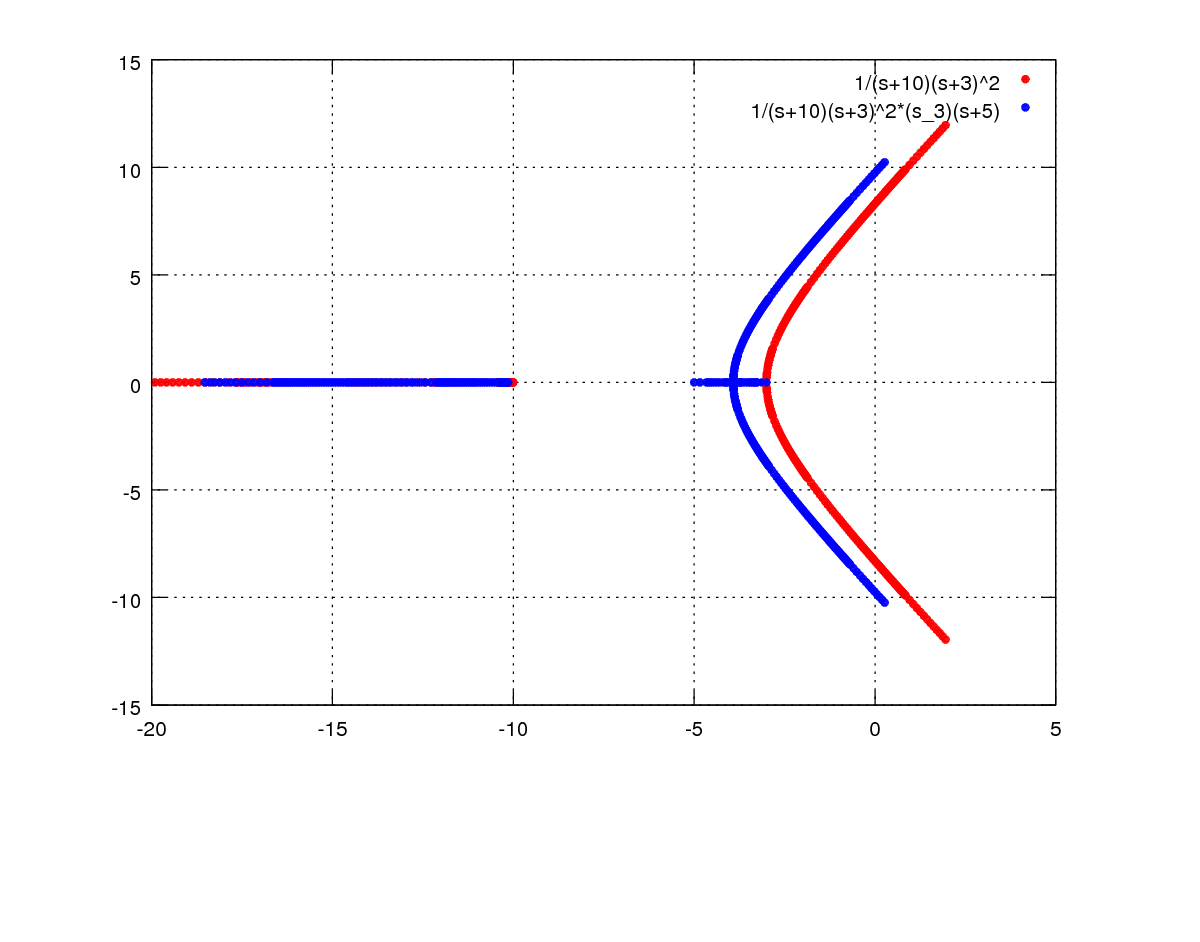
\includegraphics[width=10em]{image/lead.png}
\end{frame}
\begin{frame}
\frametitle{滞后校正}
\label{sec-4-3-2}

\begin{align*}
G(s) &=\frac{1}{(s+10)(s+3)^2}\\
G_c(s) &=\frac{10s+1}{100s+1}
\end{align*}

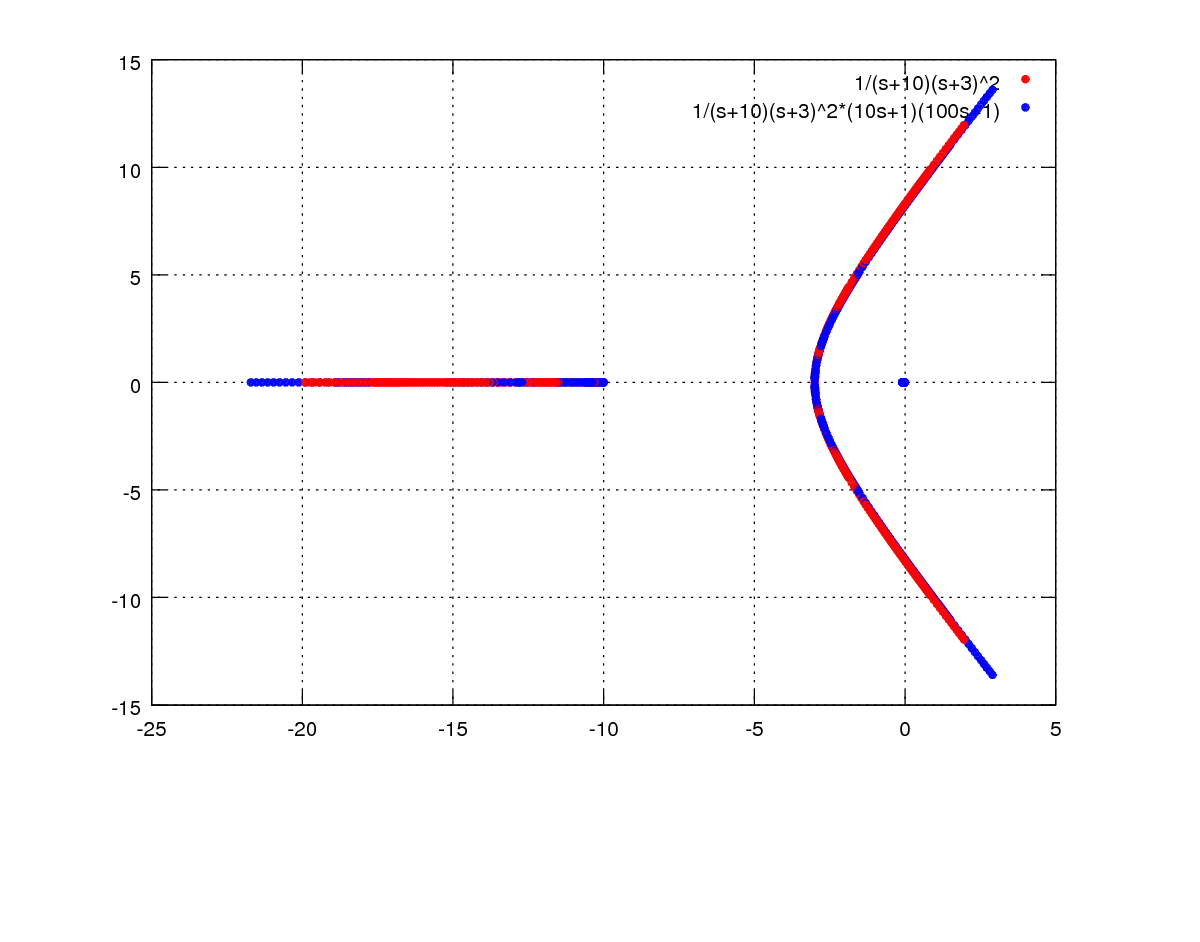
\includegraphics[width=10em]{image/lad.png}
\end{frame}

\end{document}
